\documentclass[a4paper]{article}
\usepackage[spanish]{babel}
\usepackage[utf8]{inputenc}
\usepackage{fancyhdr}
\usepackage{charter}   % tipografía
\usepackage{graphicx}
\usepackage{makeidx}

\usepackage{float}
\usepackage{amsmath, amsthm, amssymb}
\usepackage{amsfonts}
\usepackage{sectsty}
\usepackage{wrapfig}
\usepackage{listings} % necesario para el resaltado de sintaxis
\usepackage{caption}
\usepackage{placeins}
\usepackage{longtable}

\usepackage{hyperref} % agrega hipervínculos en cada entrada del índice
\hypersetup{          % (en el pdf)
    colorlinks=true,
    linktoc=all,
    citecolor=black,
    filecolor=black,
    linkcolor=black,
    urlcolor=black
}

\usepackage{color} % para snippets de código coloreados
\usepackage{fancybox}  % para el sbox de los snippets de código

\definecolor{litegrey}{gray}{0.94}

% \newenvironment{sidebar}{%
% 	\begin{Sbox}\begin{minipage}{.85\textwidth}}%
% 	{\end{minipage}\end{Sbox}%
% 		\begin{center}\setlength{\fboxsep}{6pt}%
% 		\shadowbox{\TheSbox}\end{center}}
% \newenvironment{warning}{%
% 	\begin{Sbox}\begin{minipage}{.85\textwidth}\sffamily\lite\small\RaggedRight}%
% 	{\end{minipage}\end{Sbox}%
% 		\begin{center}\setlength{\fboxsep}{6pt}%
% 		\colorbox{litegrey}{\TheSbox}\end{center}}

\newenvironment{codesnippet}{%
	\begin{Sbox}\begin{minipage}{\textwidth}\sffamily\small}%
	{\end{minipage}\end{Sbox}%
		\begin{center}%
		\colorbox{litegrey}{\TheSbox}\end{center}}



\usepackage{fancyhdr}
\pagestyle{fancy}

%\renewcommand{\chaptermark}[1]{\markboth{#1}{}}
\renewcommand{\sectionmark}[1]{\markright{\thesection\ - #1}}

\fancyhf{}

\fancyhead[LO]{Sección \rightmark} % \thesection\
\fancyfoot[LO]{\small{Cravero, Guerson, Mignanelli, Suárez}}
\fancyfoot[RO]{\thepage}
\renewcommand{\headrulewidth}{0.5pt}
\renewcommand{\footrulewidth}{0.5pt}
\setlength{\hoffset}{-0.8in}
\setlength{\textwidth}{16cm}
%\setlength{\hoffset}{-1.1cm}
%\setlength{\textwidth}{16cm}
\setlength{\headsep}{0.5cm}
\setlength{\textheight}{25cm}
\setlength{\voffset}{-0.7in}
\setlength{\headwidth}{\textwidth}
\setlength{\headheight}{13.1pt}

\renewcommand{\baselinestretch}{1.1}  % line spacing


\usepackage{underscore}
\usepackage{caratula}
\usepackage{url}
\usepackage{color}
\usepackage{clrscode3e} % necesario para el pseudocodigo (estilo Cormen)




\begin{document}
%
%\lstset{
%  language=C++,                    % (cambiar al lenguaje correspondiente)
%  backgroundcolor=\color{white},   % choose the background color
%  basicstyle=\footnotesize,        % size of fonts used for the code
%  breaklines=true,                 % automatic line breaking only at whitespace
%  captionpos=b,                    % sets the caption-position to bottom
%  commentstyle=\color{red},    % comment style
%  escapeinside={\%*}{*)},          % if you want to add LaTeX within your code
%  keywordstyle=\color{blue},       % keyword style
%  stringstyle=\color{blue},     % string literal style
%}

\thispagestyle{empty}
\materia{Teoría de las Comunicaciones}
\submateria{Segundo Cuatrimestre 2016}
\titulo{TP1: Wiretapping}
%\subtitulo{Planos de Corte (INSERTE MEJORAS)}
\integrante{Cravero, Marcos}{495/15}{marcoscravero2175@gmail.com} % por cada integrante (apellido, nombre) (n° libreta) (e-mail)
\integrante{Mignanelli, Alejandro Rubén}{609/11}{minga_titere@hotmail.com} 
\integrante{Suárez, Federico}{610/11}{elgeniofederico@gmail.com} 

\maketitle
\newpage

\thispagestyle{empty}
\vfill
%\begin{abstract}
%    \vspace{0.5cm}
%	
%
%\end{abstract}

\thispagestyle{empty}
\vspace{1.5cm}
\tableofcontents
\newpage

%\normalsize
 
\newpage

\section{Introducción}

En este trabajo práctico nos proponemos experimentar con herramientas y técnicas de uso frecuente a
nivel de red. Particularmente, la versión de traceroute basada en los mensajes echo request/reply del
protocolo ICMP. Los objetivos son múltiples. Por un lado entender los protocolos involucrados y
desarrollar nuestras propias implementaciones para afianzar los conocimientos. Por otra parte, utilizar lo hecho para analizar un ejemplo real, y poder contrastar la teoría con práctica. Para esto, se propondrá un experimento que permita cumplir con los fines recién mencionados.

%\newpage

\section{Experimentos}

\subsection{Explicación}

A lo largo de este trabajo realizaremos un experimento que consiste en ejecutar una implementación propia del traceroute sobre varios casos de estudio y poder analizar así como se va armando la ruta y que es lo que sucede en cada salto, tratando de detectar factores como por ejemplo los saltos intercontinentales.

Para poder llevar esto a cabo desarrollamos una primera herramienta, $tp2.py$, con la cual podemos realizar un traceroute a cualquier $IP$ o $URL$. \\
En la implementación utilizamos la librería $scapy$ que nos permite crear, enviar y analizar paquetes. \\
Con el objetivo de obtener información de cada salto, generamos y envíamos un paquete de tipo $ECHO$ incrementando el $TTL (Time\ To\ Live)$ desde 1 hasta alcanzar el destino solicitado o un máximo configurable. Las posibles respuestas que podemos tener para este paquete enviado son las siguientes:
\begin{itemize}
	\item $ECHO\ REPLY:$ El paquete llegó a destino. 
	\item $TIME\ EXCEEDED:$ Se realizaron tantos saltos como el $TTL$ configurado y aún no se pudo alcanzar el destino.
	\item Sin respuesta: En algunos casos directamente no recibiremos respuesta para un paquete enviado, por lo que luego de cierto $timeout$ diremos que no hemos obtenido respuesta. Esto se puede deber a que, entre otras cosas, es posible configurar un router para que no responda este tipo de paquetes y de esta forma se reduzca el tráfico en la red.
\end{itemize}

Como bien sabemos, para poder realizar un traceroute, debemos determinar mediante algún criterio un nodo para cada salto y el tiempo que implicó dicho hop.
Veamos entonces los criterios establecidos en nuestra implementación:
\begin{itemize}
	\item Elección del nodo en cada salto: Para cada $TTL$ decidimos envíar una ráfaga de paquetes y analizar sus respuestas. En caso de recibir al menos una respuesta de tipo $ECHO\ REPLY$ quiere decir que hemos alcanzado el destino, por tal motivo el nodo seleccionado será ese. \\
Por otro lado, si aún no hemos alcanzado el destino, seleccionaremos al nodo que más veces respondió $TIME\ EXCEEDED$ para el presente $TTL$.\\
Por último, puede presentarse el caso en donde no recibamos respuesta, en dicha situación simplemente continuaremos iterando sin analizar comportamiento alguno. \\
Cabe destacar que en nuestra implementación, la cantidad de paquetes a enviar por ráfaga es configurable.
	\item Cálculo del tiempo del salto: Una vez seleccionada la $IP$ del salto, ya sea por haber alcanzado el destino o por habernos quedado con la que más veces respondió, debemos establecer el tiempo que implicó realizar dicho hop. Para esto, simplemente promediamos los $RTT (Round\ Trip\ Time)$ del nodo seleccionado y restamos dicho valor al $RTT$ promedio del salto anterior. Notar que esta resta podría resultar en un número negativo, en dicho caso diremos que el salto demoró 0ms dado que carecería de sentido decir que el salto se realizó en un tiempo negativo. A lo largo del trabajo analizaremos el por qué de la aparición de dichos valores.
\end{itemize}

Para esta primer sección del experimento, decidimos establecer un $TTL\_MAX$ de 30 saltos, es decir que cortaremos la ejecución si no se alcanza el destino en, a lo sumo, 30 saltos. Por otro lado, por cada iteración de los $TTL$, se decidió emitir una ráfaga de 30 paquetes.

Una vez que obtuvimos el traceroute, y para poder analizar los saltos intercontinentales, desarrollamos otra herramienta llamada $outliers.py$. \\
En la misma, tomando como input la salida de la aplicación anterior, intentamos reconocer dichos saltos aplicando el método de detección de outliers de Cimbala. 

\newpage


Se realizará básicamente el mismo experimento sobre las páginas de 4 universidades:

\begin{itemize}
	\item Oxford
	
	\begin{itemize}
		\item Localización: Inglaterra, Oxford 
		\item Página: www.ox.ac.uk
	\end{itemize}

	\item Universidad de Sudáfrica (UNISA)
	
	\begin{itemize}
		\item Localización: Sudafrica, Pretoria
		\item Página: www.unisa.ac.za
	\end{itemize}
		 
	\item Auckland
	 
	\begin{itemize}
		\item Localización: Nueva Zelanda, Auckland 
		\item Página: www.auckland.ac.nz
	\end{itemize}

	\item Peking
	 
	\begin{itemize}
		\item Localización: China, Beijing 
		\item Página: www.pku.edu.cn
	\end{itemize}

\end{itemize}


\subsection{Consideraciones}

TENGO LA DUDA MENTAL DE SI EXPLICAR LO DE LOS CEROS ACA, O EN RESULTADOS, QUE OPINAN. 
YO LO PONDRÍA EN LAS CONCLUSIONES O POR AHÍ, POR AHORA SOLO DESCRIBAMOS QUE HICIMOS MÁS A GRANDES RASGOS PARA MI.

\newpage

\section{Resultados}
A continuación se presentarán los resultados de los experimentos.

\subsection{Captura de la Facultad}

\begin{figure}[H]
  \centering
    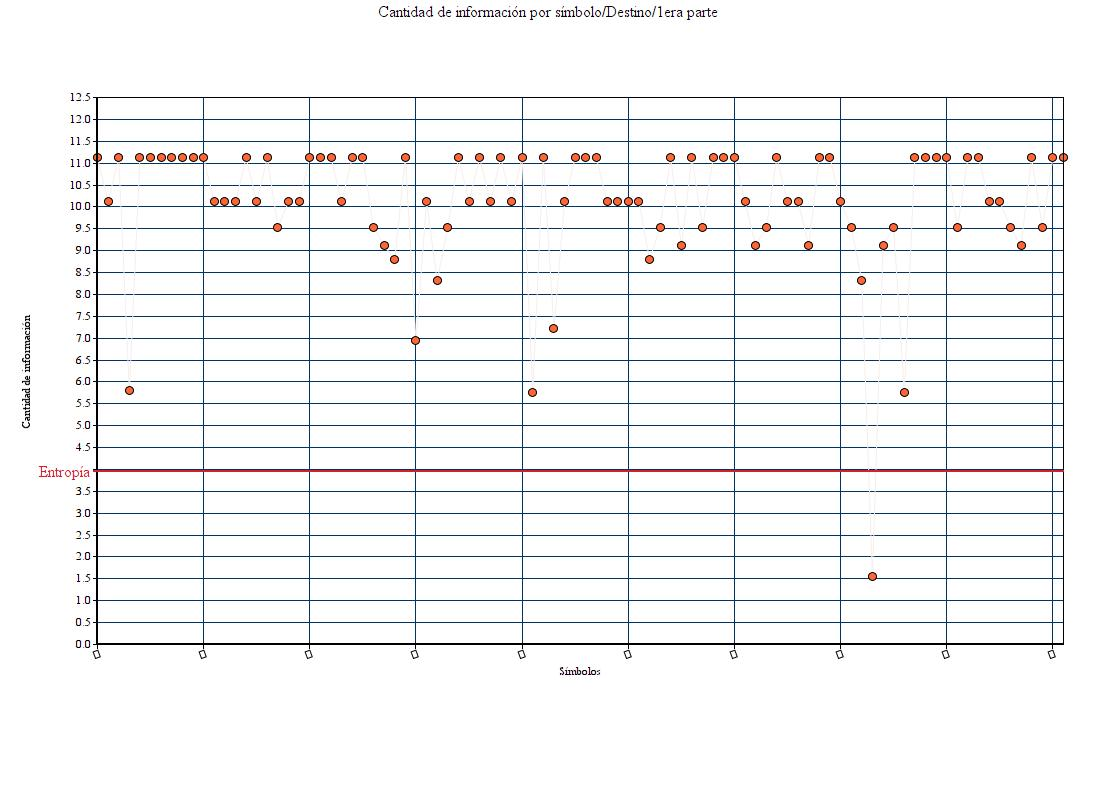
\includegraphics[scale=0.45]{imagenes/graficos/entropiaCantInf/02destino1eraParte.jpg}
  \caption{Cantidad de Información por Símbolo (Destinos) VS Entropía (Parte 1)}
  \label{fig:ejemplo}
\end{figure}
\begin{figure}[H]
  \centering
    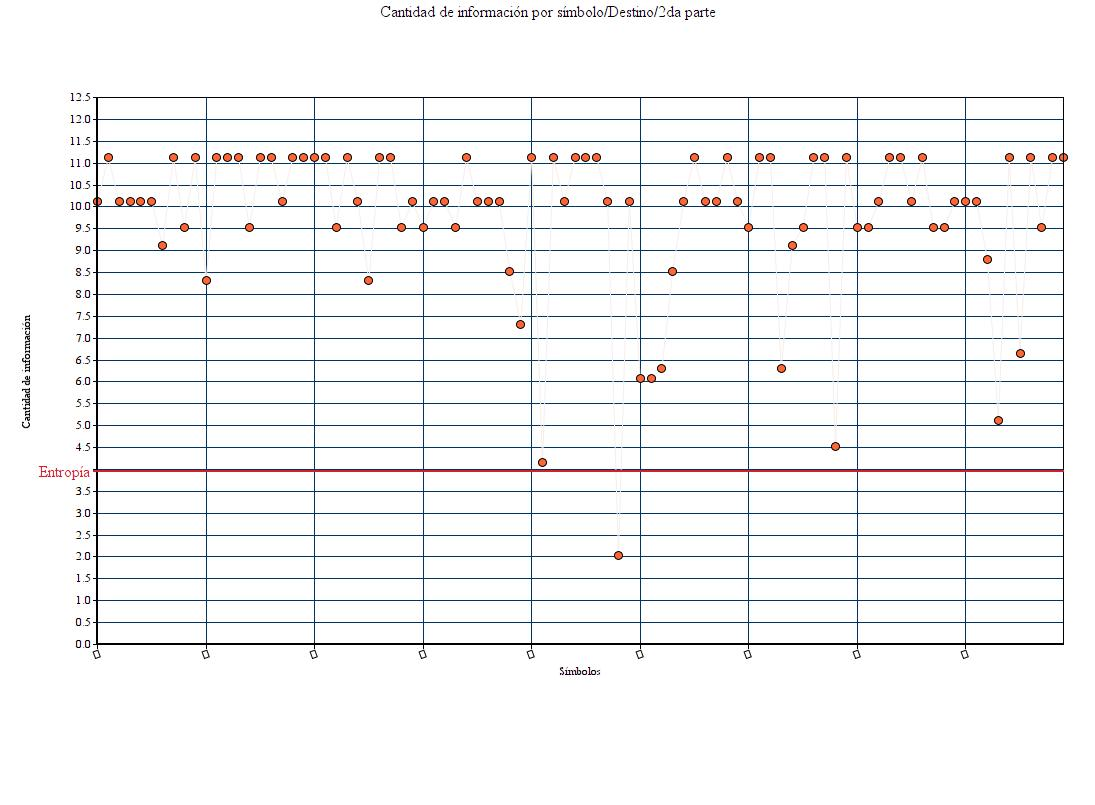
\includegraphics[scale=0.45]{imagenes/graficos/entropiaCantInf/02destino2daParte.jpg}
  \caption{Cantidad de Información por Símbolo (Destinos) VS Entropía (Parte 2)}
  \label{fig:ejemplo}
\end{figure}

En las Figuras 1 y 2, es decir, cuando se tomaron únicamente las direcciones IP de destino en el modelado, se puede ver cómo la mayor parte de los símbolos proveen una gran cantidad de información en contraste con la entropía y también cómo una minoría se destaca por proveer muy poca información. En cambio en las Figuras 3 y 4, donde se consideraron sólo las direcciones origen, si bien ocurre algo similar a lo anterior, es un poco menos acentuada la diferencia.

\begin{figure}[H]
  \centering
    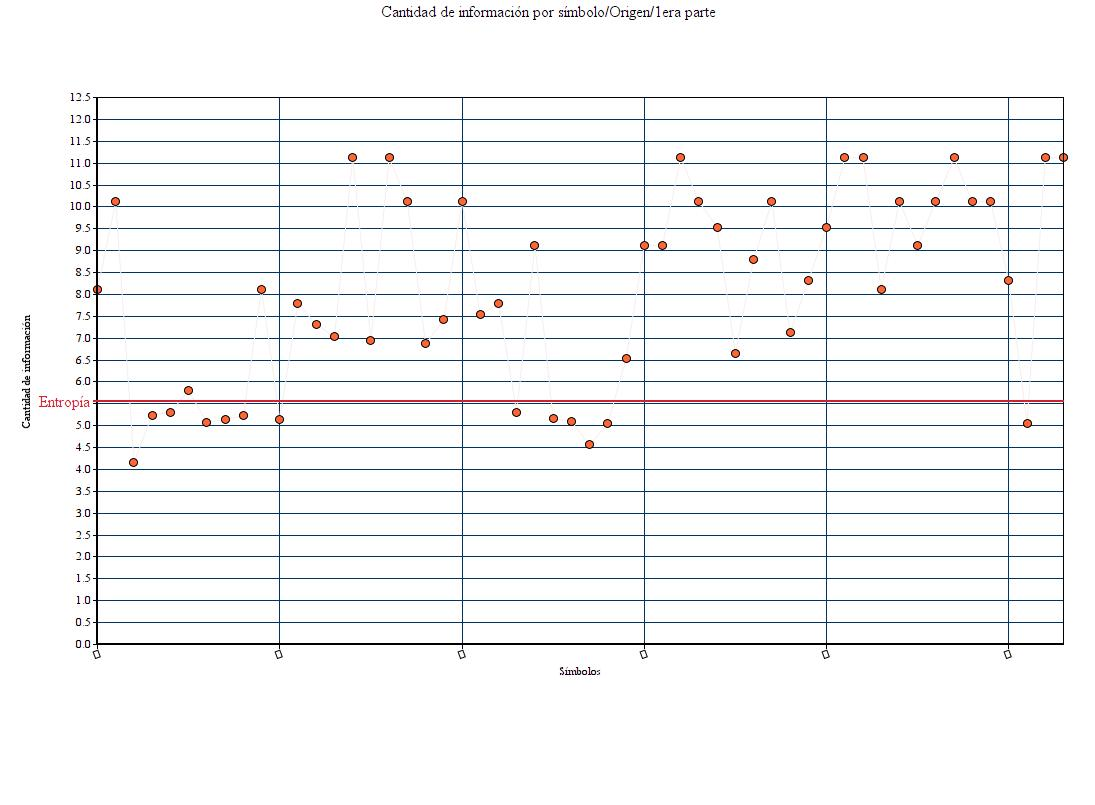
\includegraphics[scale=0.45]{imagenes/graficos/entropiaCantInf/02origen1eraParte.jpg}
  \caption{Cantidad de Información por Símbolo (Orígenes) VS Entropía (Parte 1)}
  \label{fig:ejemplo}
\end{figure}


\begin{figure}[H]
  \centering
    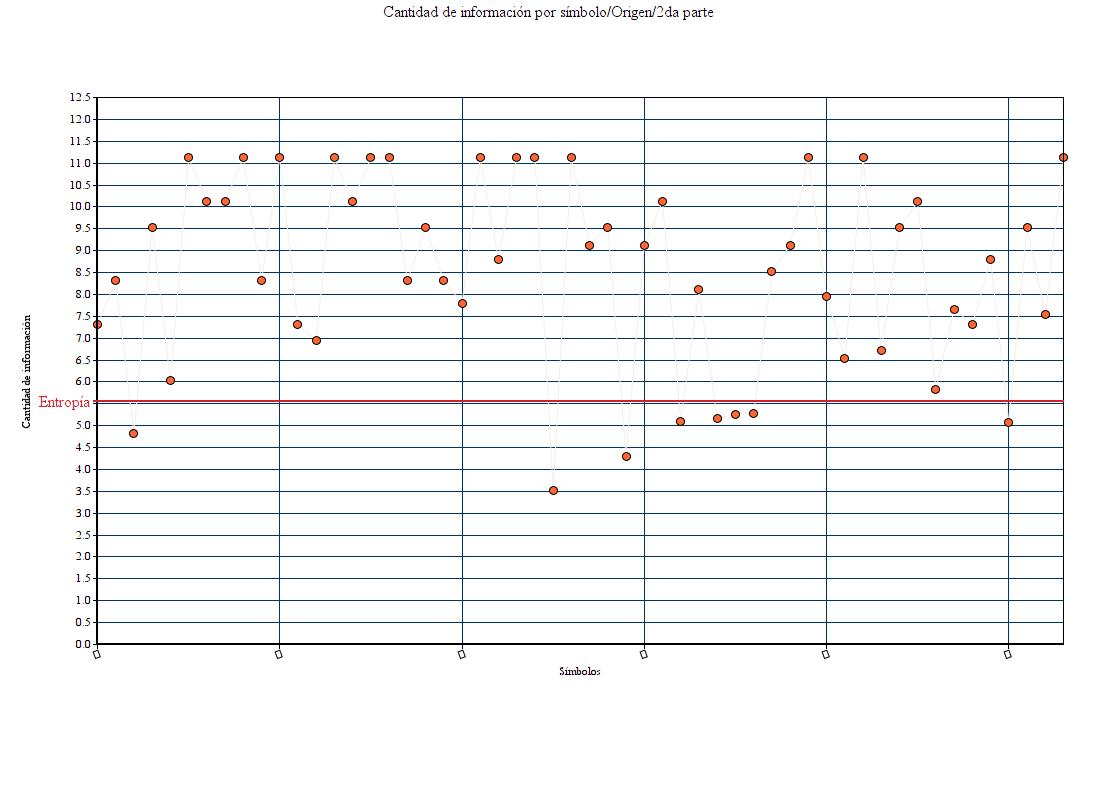
\includegraphics[scale=0.45]{imagenes/graficos/entropiaCantInf/02origen2daParte.jpg}
  \caption{Cantidad de Información por Símbolo (Orígenes) VS Entropía (Parte 2)}
  \label{fig:ejemplo}
\end{figure}

\newpage

\begin{figure}[H]
  \centering
    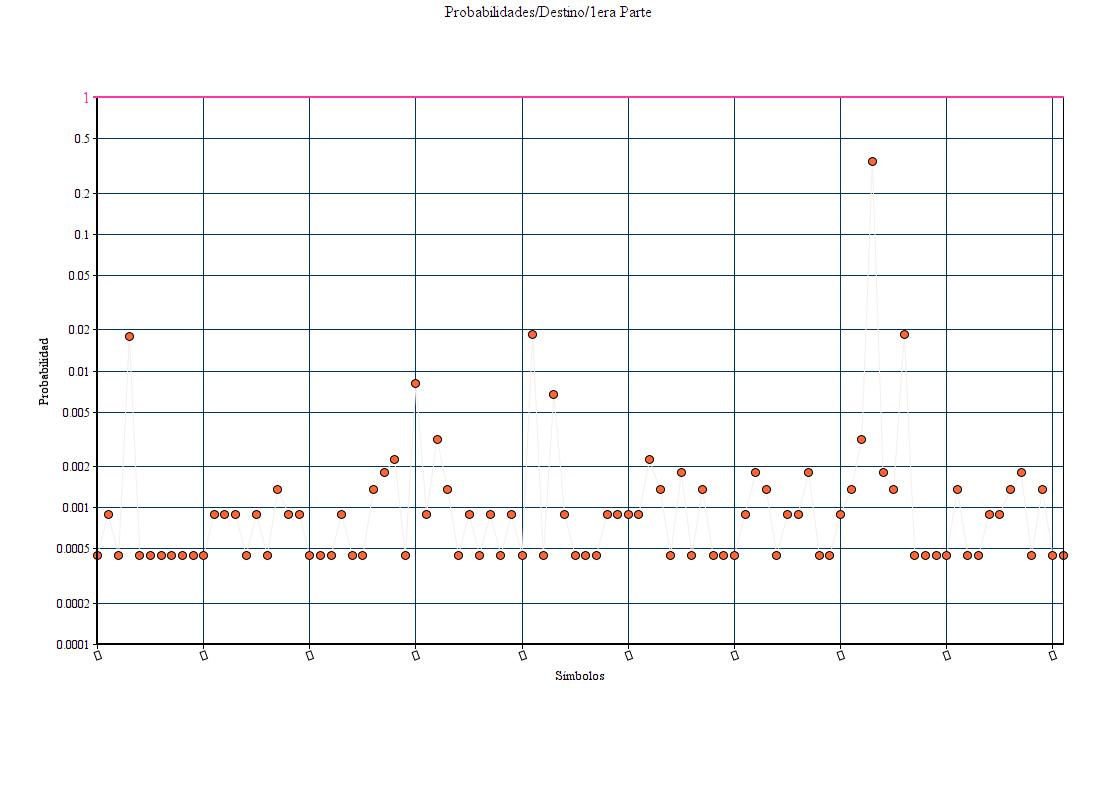
\includegraphics[scale=0.45]{imagenes/graficos/Probabilidades/02destino1eraParte.jpg}
  \caption{Probabilidad de cada Símbolo (Destinos) VS Entropía (Parte 1)}
  \label{fig:ejemplo}
\end{figure}

\begin{figure}[H]
  \centering
    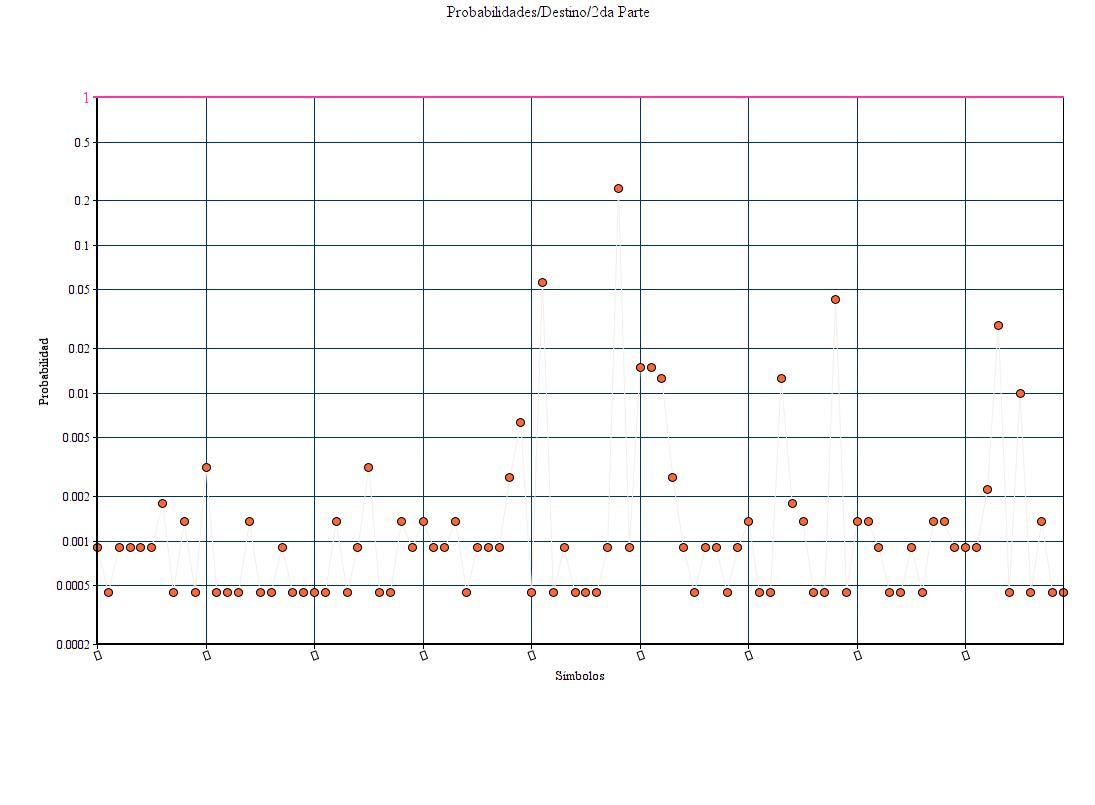
\includegraphics[scale=0.45]{imagenes/graficos/Probabilidades/02destino2daParte.jpg}
  \caption{Probabilidad de cada Símbolo (Destinos) VS Entropía (Parte 2)}
  \label{fig:ejemplo}
\end{figure}

\newpage

En el caso de las probabilidades por símbolo ocurre algo análogo a lo que pasaba con la cantidad de información por símbolo, es decir, para los destinos la mayoría tienen una probabilidad muy baja salvo unos pocos que destacan por tener una alta probabilidad, y con los orígenes se presenta algo muy similar pero con las probabilidades un poco más dispersas y no tan marcada la diferencia.

\begin{figure}[H]
  \centering
    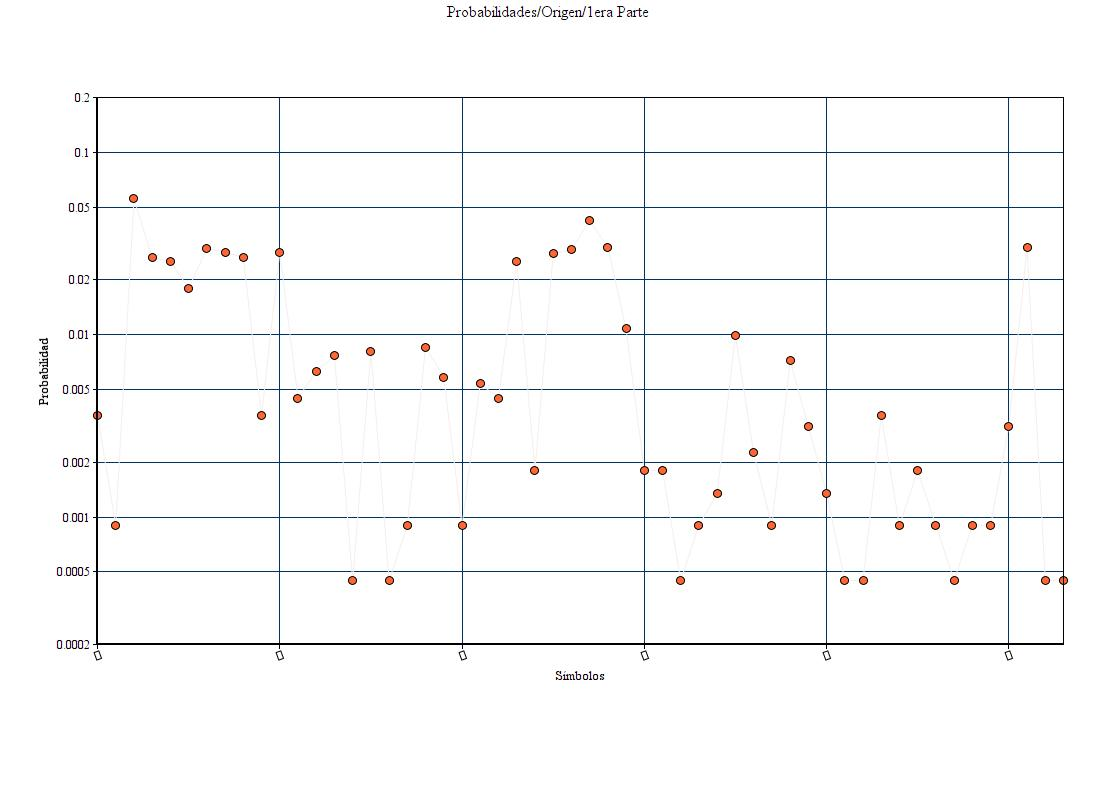
\includegraphics[scale=0.45]{imagenes/graficos/Probabilidades/02origen1eraParte.jpg}
  \caption{Probabilidad de cada Símbolo (Orígenes) VS Entropía (Parte 1)}
  \label{fig:ejemplo}
\end{figure}

\begin{figure}[H]
  \centering
    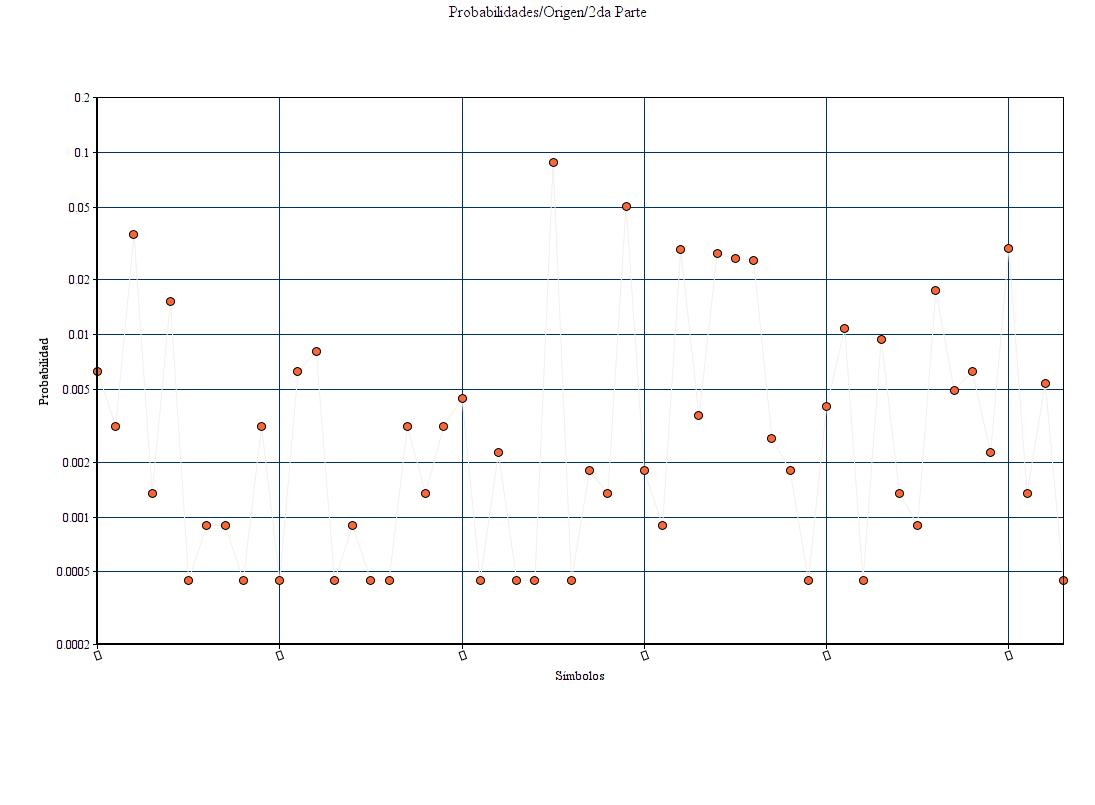
\includegraphics[scale=0.45]{imagenes/graficos/Probabilidades/02origen2daParte.jpg}
  \caption{Probabilidad de cada Símbolo (Orígenes) VS Entropía (Parte 2)}
  \label{fig:ejemplo}
\end{figure}

\begin{figure}[H]
  \centering
    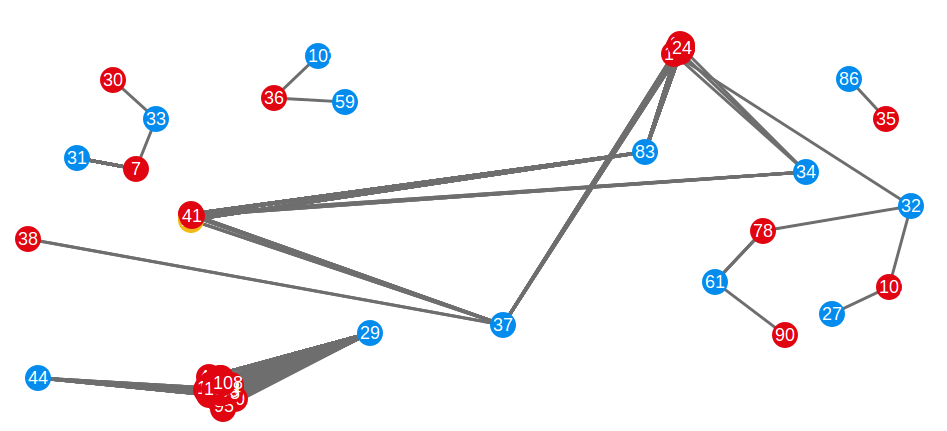
\includegraphics[scale=0.6]{imagenes/graficos/grafos/facultad.png}
  \caption{Red de conexiones entre nodos}
  \label{fig:ejemplo}
\end{figure}

Y ACÁ VA EL CHAMUYO SOBRE EL GRAFO DE LA FACULTAD Y HAY QUE MEJORAR EL CAPTION SEGURO O SACÁRSELO.

\newpage
\subsection{Captura de Starbucks}

\begin{figure}[H]
  \centering
    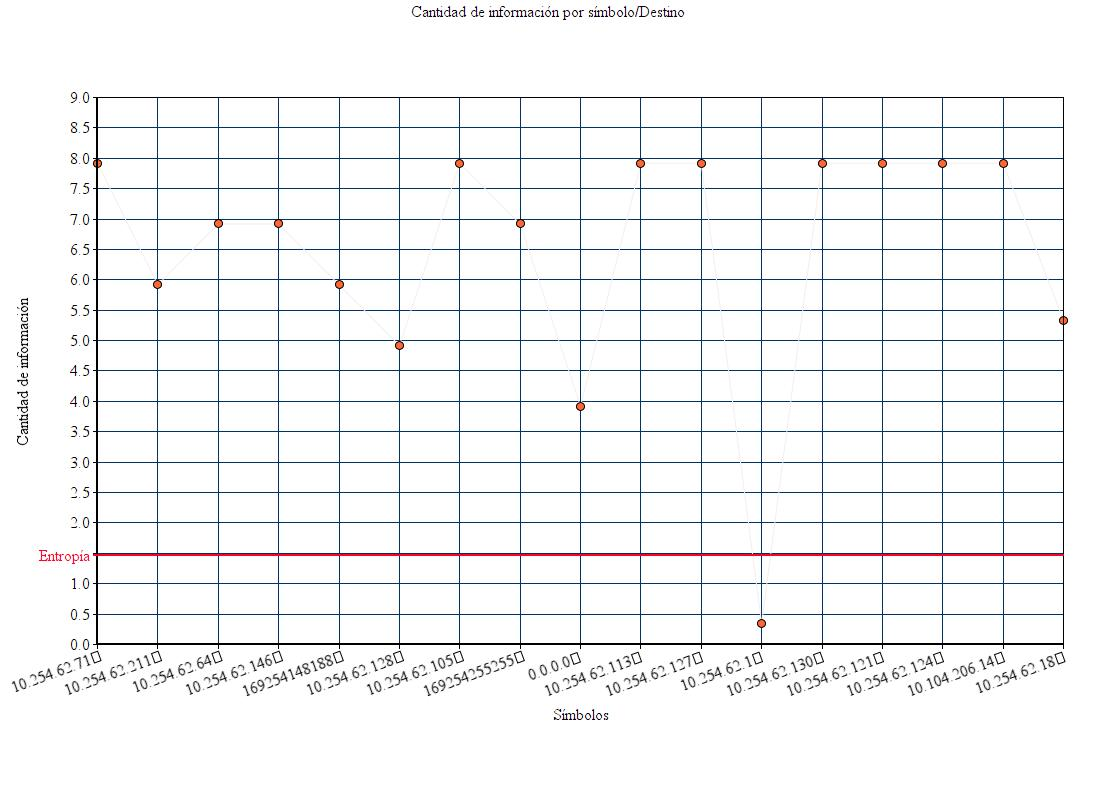
\includegraphics[scale=0.45]{imagenes/graficos/entropiaCantInf/04destino.jpg}
  \caption{Cantidad de Información por Símbolo (Destinos) VS Entropía}
  \label{fig:ejemplo}
\end{figure}

\begin{figure}[H]
  \centering
    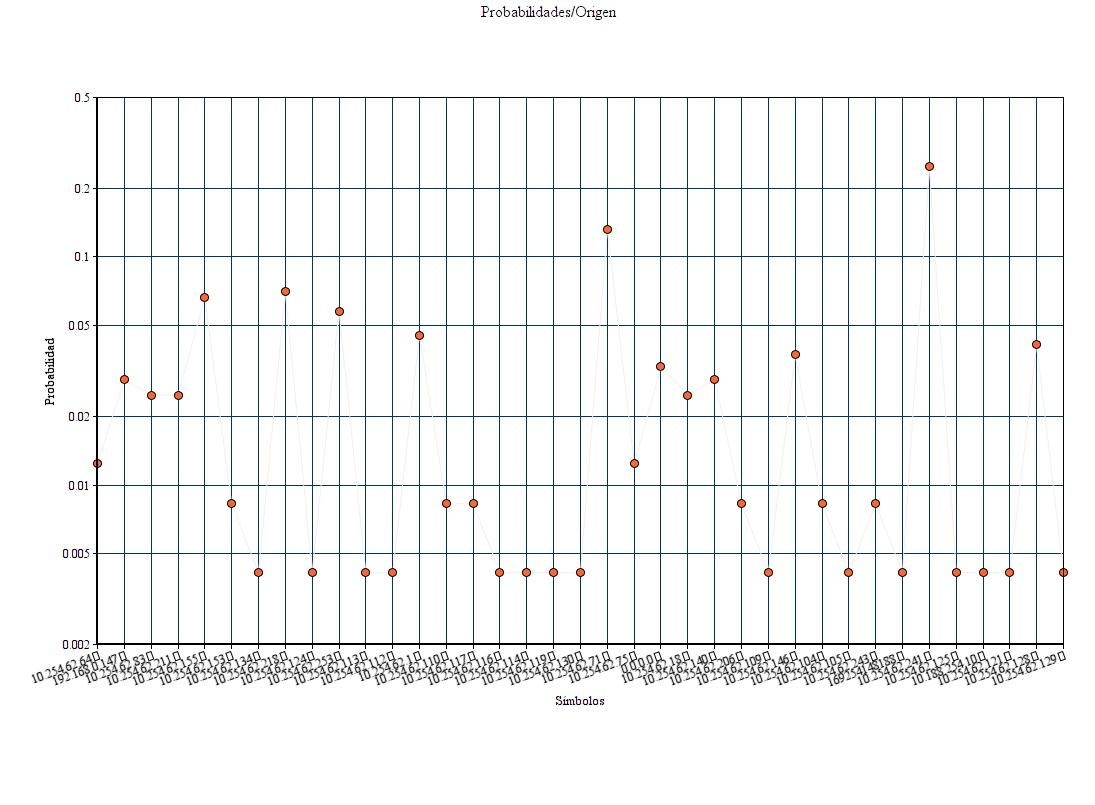
\includegraphics[scale=0.45]{imagenes/graficos/entropiaCantInf/04origen.jpg}
  \caption{Cantidad de Información por Símbolo (Orígenes) VS Entropía}
  \label{fig:ejemplo}
\end{figure}



\newpage

\section{Conclusiones}

Este fenómeno de que la mayoría de símbolos provean una cantidad información muy por encima de la entropía y sólo unos pocos por debajo, se presenta en todas las capturas. Si la entropía es una medida que indica la cantidad media de información por símbolo, ¿cómo se explica que tantos símbolos se encuentren muy por sobre la media y tan sólo una minoría por debajo? Esto puede explicarse dando un vistazo a las probabilidades de cada símbolo. Se puede ver en los resultados de las capturas que los símbolos que proveen la menor cantidad de información son aquellos con las probabilidades más altas y esto se condice con la teoría de la información, es decir, los sucesos con las probabilidades de ocurrencia más altas son los que aportan menos información (y viceversa), y a su vez si un suceso tiene 100\% de probabilidad de ocurrencia entonces se dice que su cantidad de información es $cero$. La entropía está directamente relacionada con la capacidad de distinguir símbolos, es decir, cuando la entropía es máxima todos los símbolos proveen la misma cantidad de información y son equiprobables, no hay ninguno que se distinga, y en cambio cuando los símbolos no son equiprobables y la entropía es baja se pueden distinguir aquellos símbolos que provean la menor cantidad de información, o sea, los que tengan las probabilidades más altas.
 Por otro lado, y de manera curiosa, las redes más grandes presentaron muchas similutudes en los experimentos, (sobre todo el primero y el último), mientras que la red más chica (el Cyber), se distinguía de ámbos en todo aspecto(por ejemplo, información de paquetes broadcast o el hecho de que inclusive la fuente Origen generaba símbolos distinguidos).
 Para terminar, en cuanto a la pregunta que nos hicimos al principio del proyecto sobre que fuente elegir, si aquella que representaba los destinos, o la de los orígenes, los experimentos sostuvieron que la fuente que más símbolos distinguía era la de destino, probablemente por los gateaway de las redes.

\newpage

\end{document}

